\documentclass{beamer}

\RequirePackage{beamerthemesplit}
\RequirePackage[polish]{babel}
\RequirePackage[utf8]{inputenc}
\RequirePackage[T1]{fontenc}
\RequirePackage{times}
\RequirePackage{comment}
\RequirePackage{longtable}
\RequirePackage{url}
\RequirePackage{tabularx}
\RequirePackage{hyperref}
\RequirePackage{indentfirst}
\usepackage{listings}
\usepackage{verbatim}

\usetheme{Madrid}
\usecolortheme{seahorse}

\title[Memory management in Python]{Memory management in Python - how it works and is it worth messing with it?}
\subtitle{Is it possible to have a memory leak in Python? What is the performance cost of garbage collector? When can I run into problems with memory and how can I solve them?}
% don't know if i can put company logo on the repo, so commenting it out
%\author[Maciej Pytel]{Maciej Pytel\\ \includegraphics[height=0.2\textheight]{codi.jpg}\vspace{-4ex}}
\author[Maciej Pytel]{Maciej Pytel}
\date{02/03/2015}

\begin{document}

\begin{frame}
  \begin{titlepage}
  \end{titlepage}
\end{frame}

\begin{frame}
    \frametitle{About me}
    Software developer @ CodiLime. I code (mainly) in Python. I like to know how stuff works "inside".
\end{frame}

\begin{frame}
    \frametitle{Disclaimer}
    \begin{block}{Which Python?}
        This talk is about Python 2.7.\\
        By ''Python'' I mean CPython.
    \end{block}
    \begin{block}{Examples}
        \url{https://github.com/MaciekPytel/python-memory-talk}
    \end{block}
\end{frame}

\section*{Agenda}
    \begin{frame}
      \tableofcontents
    \end{frame}

\setcounter{section}{0}
\section{Just a bit of theory}
\frame\sectionpage
    \begin{frame}
        \frametitle{Reference counting}
        \begin{itemize}
            \item Every object has a reference counter.
            \item When the counter reaches 0 the object is \textit{immediately} deallocated.
            \item What about reference cycles?
        \end{itemize}
    \end{frame}

    \begin{frame}
        \frametitle{Garbage collector}
        Mission: delete objects in unreacheable reference cycles.\\
        Solution: garbage collector.
        \begin{itemize}
            \item Automatically run by Python interpreter every once in a while.
            \item Doesn't explicitly deallocate any objects - just breaks reference cycles.
            \item Freezes the process for garbage collection.
            \item Expensive: cost is (at least) linear with regard to the number of references in program.
        \end{itemize}
    \end{frame}

    \begin{frame}
        \frametitle{Generational GC}
        \begin{block}{Weak generational hypothesis}
            Most objects live either for a very short or a very long time.
        \end{block}
        \vfill
        \begin{center}
            Can this help us optimise GC?
        \end{center}
    \end{frame}

    \begin{frame}
        \frametitle{Generational GC}
        \begin{itemize}
            \item Divide objects into 3 generations (0, 1, 2).
            \item Each newly allocated object is added to generation 0.
            \item Long living objects are promoted to higher generations.
            \item Generation 0 is made of relatively few objects with relatively large chance of being ready for deallocation (according to weak generational hypothesis).
        \end{itemize}
    \end{frame}

    \begin{frame}
        \frametitle{Generational GC}
        \begin{itemize}
            \item n-th generation garbage collection analyses objects of generation 0..n.
            \item Any object that survived n-th generation collection is promoted to generation n + 1 (technically min(2, n + 1)).
            \item 0-th generetion collection is cheap and done often.
            \item Higher generation collections are more expensive and performed much less often.
        \end{itemize}
    \end{frame}

    \begin{frame}
        \frametitle{Weak references}
        \begin{itemize}
            \item Weak reference is a reference which doesn't increase reference counter of the object it points to.
            \item Existence of weak reference doesn't prevent deallocation of its target.
            \item In Python provided by \textit{weakref} module.
            \item Dereferencing weak reference to deallocated object yields None.
        \end{itemize}
    \end{frame}


\section{Why is it worth knowing this stuff? What (and how) can we do?}
\frame\sectionpage
\subsection{Example: RESTful server}
\frame\subsectionpage
    \begin{frame}
        \frametitle{Experiment}
        \begin{itemize}
            \item Server:
            \begin{itemize}
                \item Flask-RESTful + gunicorn.
                \item Domain made of 2 classes: Task and Subtask.
                \item Natural one-to-many relationship (Each Task has multiple Subtasks).
                \item Simple API supporting creation, retrieval and deletion of Tasks and Subtasks.
            \end{itemize}
            \item Test: run a bunch of clients sending requests in a loop and measure server performance.
        \end{itemize}
    \end{frame}

    \begin{frame}[fragile]
        \frametitle{Task}
        \begin{semiverbatim}
class Task(object):
    def __init__(self, name):
        self.name = name
        self._subtasks = \{\}

    def add_subtask(self, name):
        self._subtasks[name] = Subtask(name, self)

    def get_subtask(self, name):
        return self._subtasks.get(name, None)
        \end{semiverbatim}
\end{frame}
% the above can't be intended or it won't compile, wtf :s

    \begin{frame}[fragile]
        \frametitle{Subtask version 1}
        \begin{semiverbatim}
class Subtask(object):
    def __init__(self, name, task):
        self.name = name
        self._task = task

    def get_task(self):
        return self._task
        \end{semiverbatim}
\end{frame}
% the above can't be intended or it won't compile, wtf :s

    \begin{frame}
        \frametitle{REST API}
        \begin{itemize}
            \item \textbf{GET /tasks/\{task\_id\}/} - return all Subtasks corresponding to a given Task
            \item \textbf{PUT /tasks/\{task\_id\}/} - create a Task with a given id
            \item \textbf{DELETE /tasks/\{task\_id\}/} - delete a Task and all corresponding Subtasks
            \item \textbf{GET /subtasks/\{subtask\_id\}/} - return a Subtask and its parent Task
            \item \textbf{PUT /subtasks/\{task\_id\}/\{subtask\_id\}} - create a Task with a given id and assign it to a Task
        \end{itemize}
    \end{frame}

    \begin{frame}
        \frametitle{Results}
        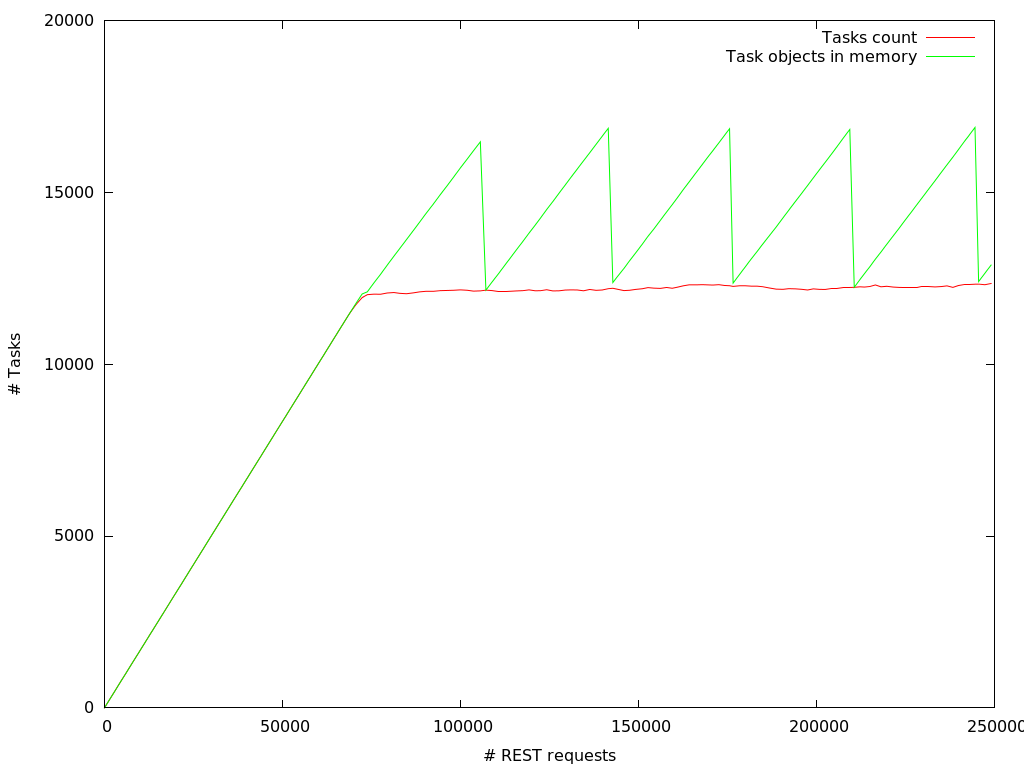
\includegraphics[height=0.8\textheight]{gc_tasks.png}
    \end{frame}

    \begin{frame}[fragile]
        \frametitle{Subtask version 2}
        \begin{semiverbatim}
import weakref

class Subtask(object):
    def __init__(self, name, task):
        self.name = name
        \alert{self._task = weakref.ref(task)}

    def get_task(self):
        return self._task()

        \end{semiverbatim}
\end{frame}
% the above can't be intended or it won't compile, wtf :s

    \begin{frame}
        \frametitle{Results?}
        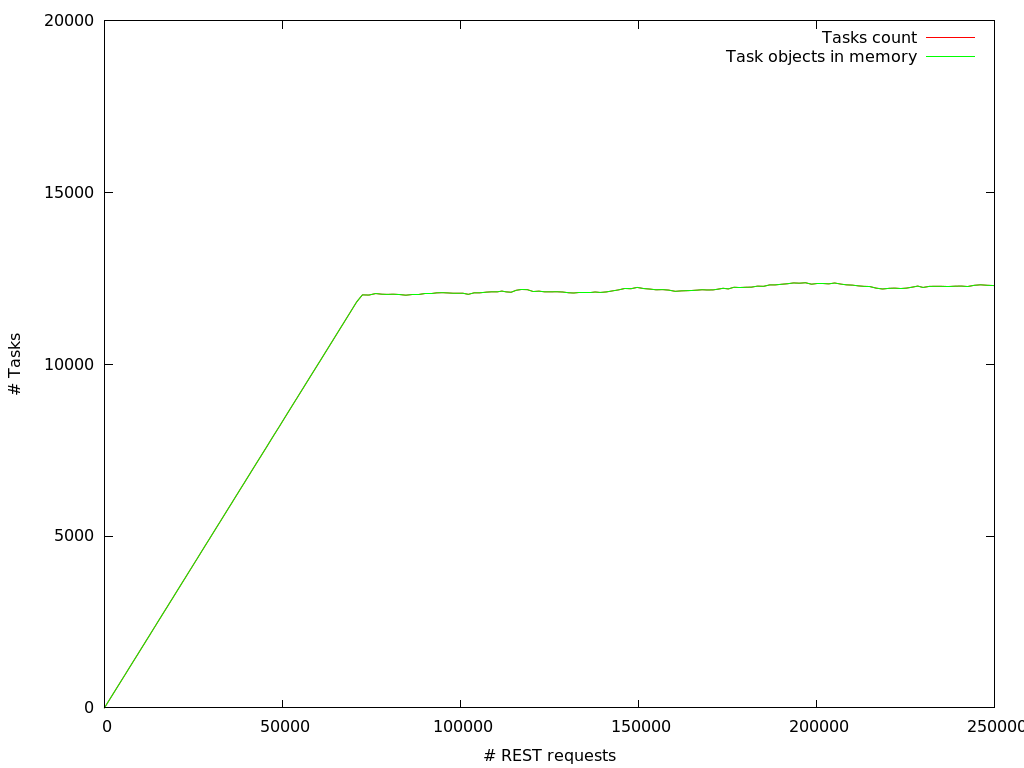
\includegraphics[height=0.8\textheight]{wr_tasks.png}
    \end{frame}

    \begin{frame}
        \frametitle{Results}
        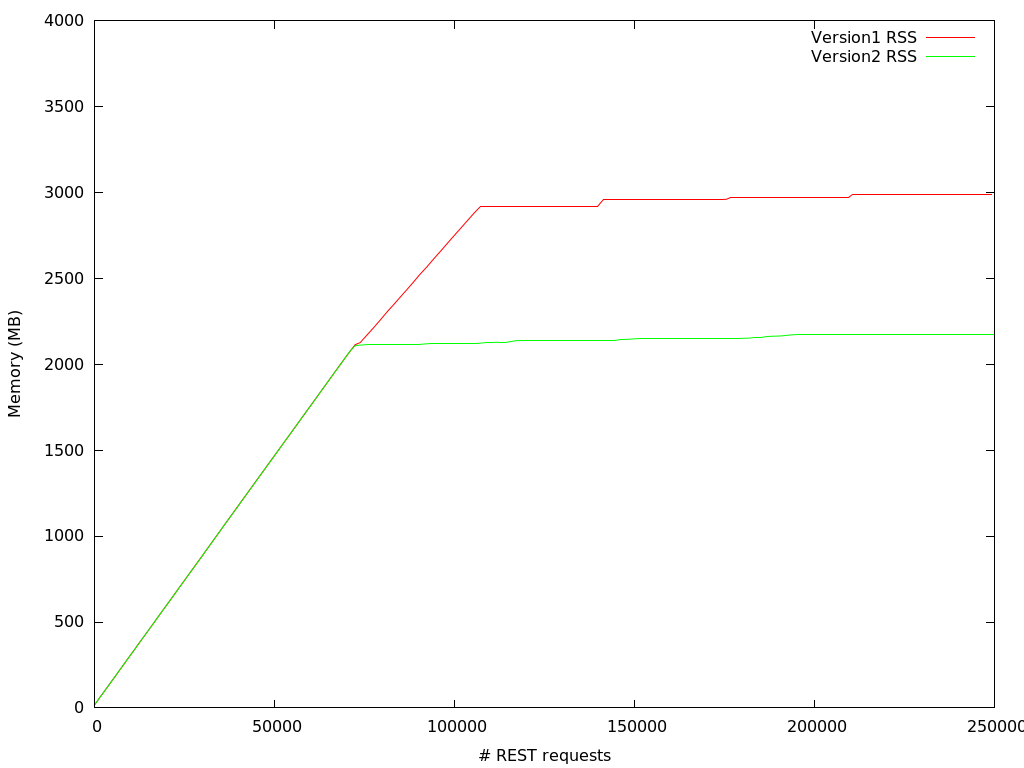
\includegraphics[height=0.8\textheight]{mem_usage.png}
    \end{frame}

    \begin{frame}
        \frametitle{Results}
        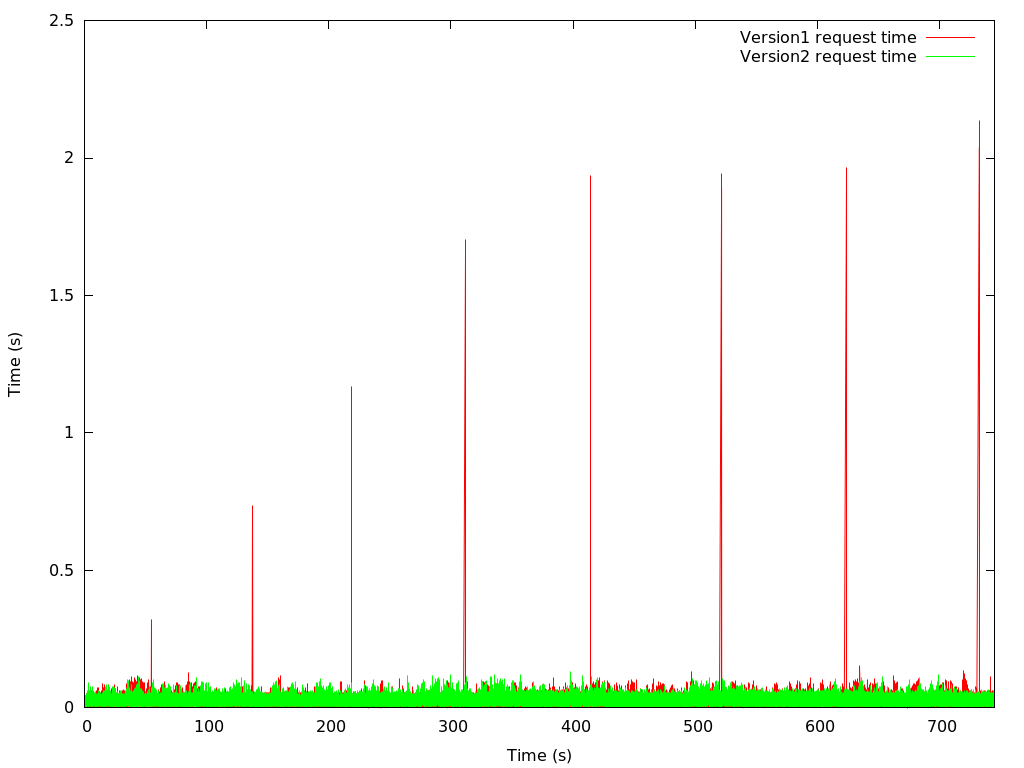
\includegraphics[height=0.8\textheight]{request_time.png}
    \end{frame}

    \begin{frame}
        \frametitle{What have we learned?}
        \begin{itemize}
            \item Relying on GC is expensive.
            \item Specifically 2nd generation GC takes a long time (2-2.5s in example server).
            \item Lower generation collections are significantly cheaper (no noticeable impact on request time for client).
            \item 2nd generation collection is run very rarely.
            \item Python is able to reuse freed memory, but it doesn't seem to return it to OS.
        \end{itemize}
    \end{frame}

    \begin{frame}
        \frametitle{Freeing memory}
        \begin{itemize}
            \item Python uses its own memory allocator (we'll skip the details).
            \item Allocator can return the memory to OS\textsuperscript{*}, but:
            \begin{itemize}
                \item Memory is allocated in blocks and only released once all objects in a block are deallocated (fragmentation!).
                \item Many objects are returned to pool for reuse (ex. tuples).
                \item Memory allocated for integers will never be freed or used for anything else.
                \item Same with floats.
                \item ...
            \end{itemize}
        \end{itemize}
    \end{frame}

    \begin{frame}
        \frametitle{Conclusion}
        If our program is having memory problems we may:
        \begin{itemize}
            \item Remove references to objects as soon as we don't need them anymore.
            \item Avoid \textit{unnecessary} reference cycles.
            \item In most cases when they are necessary we can use weakrefs.
            \item Or explicitly break the cycle when we don't need the object anymore (ex. by defining and calling \textit{delete} method).
            \item \textit{xrange} instead of \textit{range} in long loops makes a difference. Seriously, use generators.
        \end{itemize}
    \end{frame}

\subsection{Memory leaks}

\frame\subsectionpage
    \begin{frame}
        \frametitle{Memory leaks}
        There are a few possible reasons for leaks:
        \begin{enumerate}
            \item Memory leak in c/c++ module.
            \item Memory allocated for integers or floats will never be freed or used for anything else.
            \item ''Forgotten'' references.
            \item Garbage collector won't free \textit{any} object in a cycle where at least a single object defines a finalizer (\textit{\_\_del\_\_}).
        \end{enumerate}
    \end{frame}

    \begin{frame}
        \frametitle{''Forgotten'' references}
        There are a few places where unexpected references can hide and keep your objects alive:
        \begin{enumerate}
            \item sys.exc\_info() returns information about last exception handled in this stack frame. Part of this information is a traceback object containing whole stack state at the time of exception. If you catch an exception in your main loop: Oops.
            \item Closures, functools.partial, etc.
        \end{enumerate}
    \end{frame}

    \begin{frame}
        \frametitle{Finalizer (\_\_del\_\_)}
        \begin{itemize}
            \item If an object defines \_\_del\_\_ method it will be called just before object deallocation.
            \item Object can create a reference to itself in \_\_del\_\_ - this will prevent deallocation.
            \item \textbf{GC will never deallocate an object defining \_\_del\_\_!}
            \item In other words the whole cycle containing such an object will never be broken.
            \item \textbf{Warning:} \_\_del\_\_ is used in many existing libraries (including Python standard library!).
        \end{itemize}
    \end{frame}

    \begin{frame}
        \frametitle{Finalizer}
        As we can see finalizers can cause problems. How do we deal with them?
        \begin{itemize}
            \item Don't use finalizers. Context manager (''with'') is almost always a better solution.
            \item If you really need a finalizer - make sure it's never a part of reference cycle (think decomposition).
            \item As a last resort: weakref.ref takes an optional callback parameter. This callback will be called after the object is deallocated. Problem: once the callback gets invoked the object no longer exists, so we need to keep the necessary state externally.
        \end{itemize}
    \end{frame}

    \begin{frame}[fragile]
        \frametitle{weakref based finalizer}
        \begin{semiverbatim}
class FileWrapper(object):
    _weakrefs = set()

    @classmethod
    def _delegated_close(cls, file_object, w):
        file_object.close()
        cls._weakrefs.remove(w)

    def __init__(self, name, mode):
        self._f = open(name, mode)
        self._weakrefs.add(weakref.ref(
            self,
            functools.partial(self._delegated_close,
                self._f)))
        \end{semiverbatim}
\end{frame}

\section{A few useful tools}
\frame\sectionpage

    \begin{frame}
        \frametitle{pdb}
        \begin{center}
            Debugger, part of Python standard library. Allows you to inspect the state of your program, execute code and evaluate expressions in any stack frame. The basic Python debugging tool.
        \end{center}
    \end{frame}

    \begin{frame}
        \frametitle{gc}
        Python standard library module.
        \begin{itemize}
            \item \textbf{gc.collect(generation=2)} - trigger GC manually.
            \item \textbf{gc.enable() / gc.disable()} - enable/disable automatic GC.
            \item \textbf{gc.garbage} - a list of all objects that should be deleted, but define \_\_del\_\_ method and are a part of reference cycle.
            \item You can set debugging flags, ex. to print GC statistics with variable level of details.
            \item Can give you a full list of objects referring a given object.
        \end{itemize}
    \end{frame}

    \begin{frame}
        \frametitle{objgraph}
        Simple library for analysys and visulisation of reference graph. Very useful when looking for memory leaks.
        \begin{itemize}
            \item Available via pip.
            \item Visualise reference graphs.
            \item Count objects in memory by type.
            \item Also display change in number of objects of given type in time.
            \item Sufficient to diagnose 99\% of memory problems.
        \end{itemize}
    \end{frame}

    \begin{frame}
        \frametitle{objgraph}
        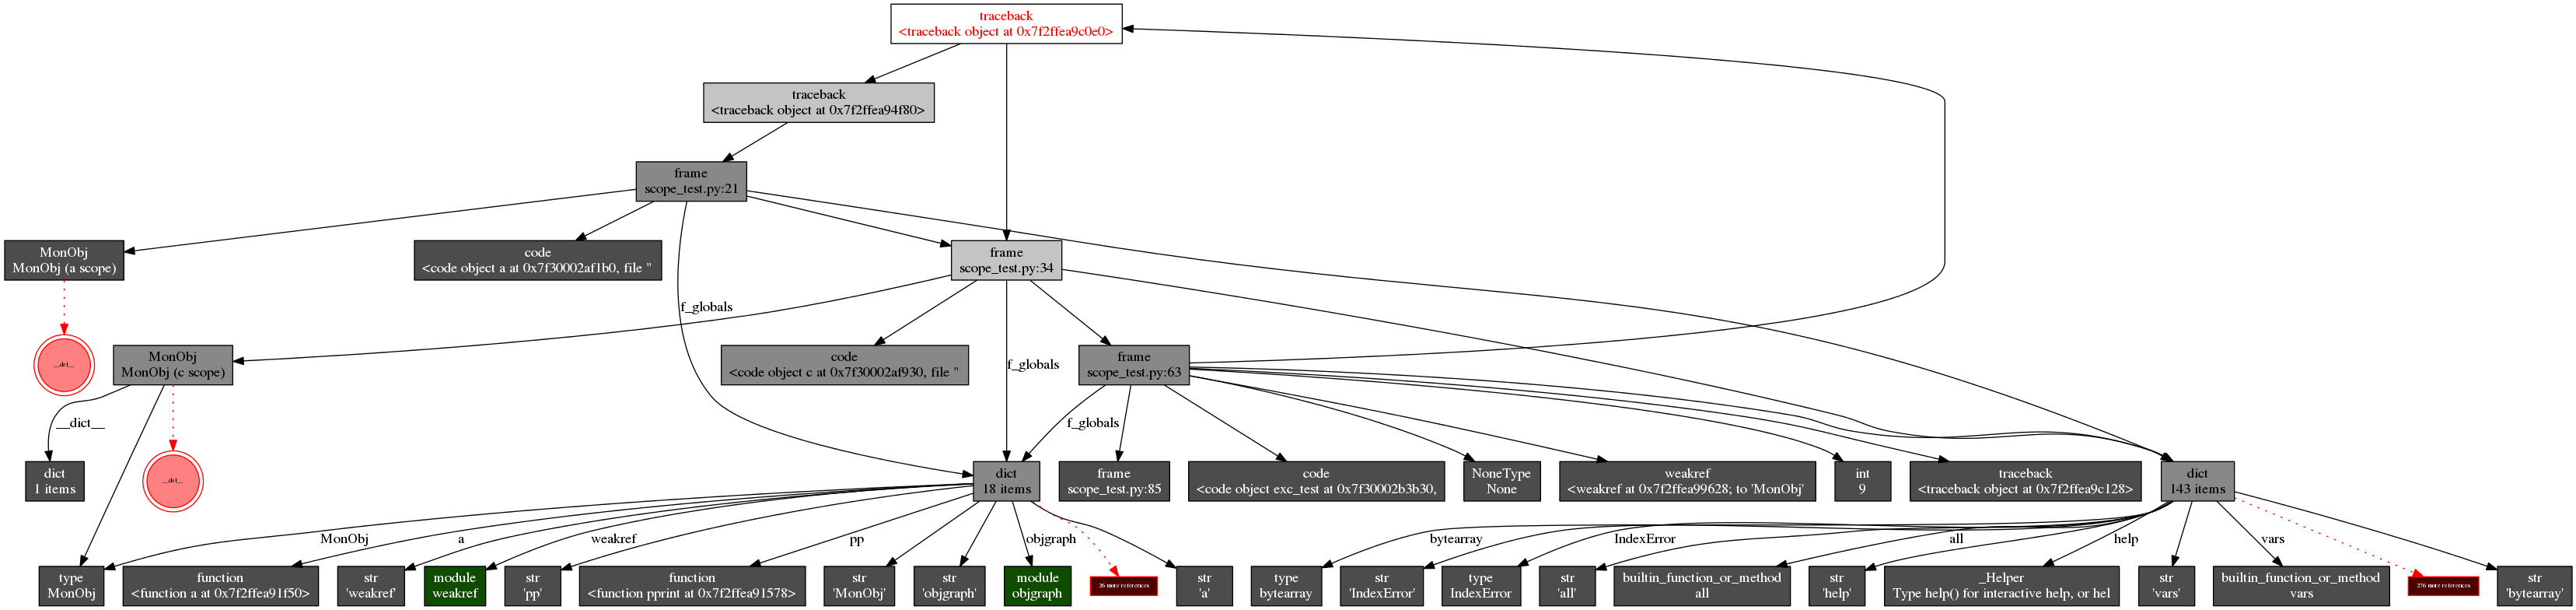
\includegraphics[height=0.3\textheight]{objgraph_example.png}
    \end{frame}

    \begin{frame}
        \frametitle{guppy/heapy}
        \begin{itemize}
            \item Memory profiler.
            \item Incredible number of available functions: analyse paths in reference graph, reference graph spanning trees (!), grouping objects by various equality relationships (ex. class, module the originates from), ...
            \item Provides hooks for tracking objects defined in C module.
            \item Steep learning curve, not the best documentation and lack of good tutorials.
            \item For this 1\% of situations when objgraph simply isn't enough :)
        \end{itemize}
    \end{frame}

\section{More theory, or how it all works?}
\frame\sectionpage

    \begin{frame}
        \frametitle{Generations}
        \begin{itemize}
            \item Each generation is a doubly-linked list.
            \item Each newly allocated object is added to generation 0.
            \item Before n-th generation GC lower generations' lists are merged to n-th generation list.
            \item After n-th generation GC is done surviving objects' list is merged to generation n + 1.
        \end{itemize}
    \end{frame}

    \begin{frame}
        \frametitle{GC algorithm}
        \begin{enumerate}
            \item (For generation 1 and 2) Merge lower generation into current generation (doubly-linked list merge).
            \item Iterate over objects on the list. Check all outgoing references (non-recursively) - if they point to other objects on the list decrease target's refcount.
            \item Iterate over objects on the list. Move any object with refcount equal to 0 to a new \textit{unreacheable} list.
            \item Iterate over objects remaining on the original list. Check all outgoing references and move any target on \textit{unreacheable} list back to the original list.
            \item Restore original refcounts on all objects.
            \item Merge original list to generation n + 1.
            \item For each object on \textit{unreacheable} list remove all references originating from that object.
        \end{enumerate}
    \end{frame}

    \begin{frame}
        \frametitle{Example}
        \begin{center}
            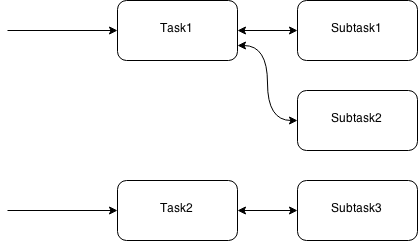
\includegraphics[height=0.5\textheight]{graph_initial.png}
        \end{center}
    \end{frame}

    \begin{frame}
        \frametitle{Example}
        \begin{center}
            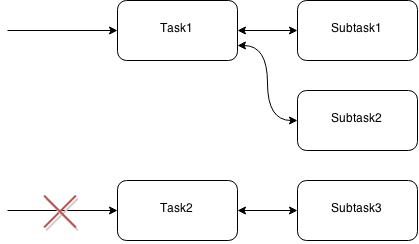
\includegraphics[height=0.5\textheight]{graph_remove.png}
        \end{center}
    \end{frame}

    \begin{frame}
        \frametitle{GC - visualisation}
        \begin{center}
            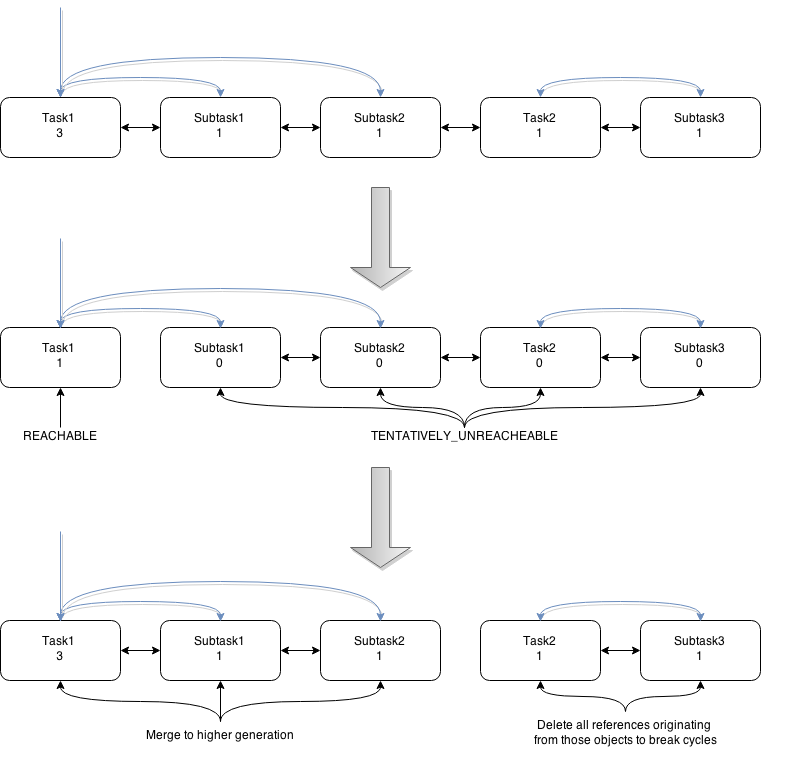
\includegraphics[height=0.8\textheight]{full_gc_drawing.png}
        \end{center}
    \end{frame}

    \begin{frame}
        \frametitle{Notes}
        \begin{itemize}
            \item The above is the idea of the algorithm. The real implementation is a bit more complex.
            \item Details in Python source /Modules/gcmodule.c - very well commented.
        \end{itemize}
    \end{frame}

    \begin{frame}
        \frametitle{Quote}
        \begin{quote}
            Programmers waste enormous amounts of time thinking
            about the speed of noncritical parts of their programs (...). We
            should forget about small efficiencies, say about 97\% of the
            time: premature optimization is the root of all evil. Yet we
            should not pass up our opportunities in that critical 3\%.
        \end{quote}
        \hspace*\fill{- Donald Knuth}
    \end{frame}

\end{document}
